% !TEX root = main.tex
\section{StopInfo Contributor Values}
\label{sec:contributor-values}

Our initial work with the StopInfo system focused on the values associated with blind and low vision transit riders, the primary group for which StopInfo was designed \cite{campbell-2014}. However, the system would not be useful to this stakeholder group (or StopInfo users in general) if the information provided is not reliable, meaning that it must be both \emph{accurate} and \emph{complete}, which were discussed in the StopInfo section previously.

To help bolster the completeness and accuracy of StopInfo information, we decided to investigate the motivations and values associated with contributing information to StopInfo with former and potential contributors, in hopes of being able to increase and sustain the level of contributions all the while promoting high-quality submissions.   

\subsection{Formative Study}
During the summer of 2014 (five months after StopInfo had been deployed), we performed a formative study by surveying 15 StopInfo contributors and 31 non-contributors. The survey addressed the basic usability of our current StopInfo system\footnote{At the time, we had just incorporated the top contributor list and badge system, and no one participating in the survey reported having noticed them before, so we do not believe these aspects of the system were well addressed.} and asked about potential motivations for contributing information about bus stops. 

We also spoke to nine participants in follow-up semi-structured interviews about their contributions to other projects that involve crowd or community sourcing, and their views of the StopInfo project as a whole. To us, one of the more interesting findings from this study was the emphasis on wanting to interact with and benefit the community, although it was not clear to us what who was meant by `community' here.

\subsection{Optimal Conditions for Submitting}
From these results, we also learned what might entail optimal (i.e. lowest cost) conditions for contributing information to StopInfo. That is, intrinsic motivating factors and incentives aside, StopInfo contributors and non-contributors alike reported that they would be most \emph{able} to contribute to StopInfo if:
\begin{itemize}[leftmargin=8mm]
\item It is easy enough to get to StopInfo within the OneBusAway application.
\item They are aware of the presence of StopInfo while waiting at a bus stop.
\item They have downtime while waiting for their bus.
\item The form is quick to fill out and the categories of information are unambiguous.
\end{itemize}

The above cases mostly center around system usability, opportunity to enter information, and salience. In terms of conditions that we can directly impact, we are continually working to improve the salience and ease of access of the StopInfo feature within OneBusAway, as well as highlight the option to edit stop information while the individual is viewing that stop's information page. Outside of the system itself, we are also participating in outreach (e.g., attending relevant events and sending out press releases). We would also like to put up physical notices (along with Braille translations) at bus stops around Seattle to call attention to the StopInfo feature.

\subsection{Incentivizing Higher Cost Submissions}

Additionally, we learned that some contributors would be willing to submit information at a higher cost given enough incentive and/or intrinsic motivation. Cases in which the cost for submitting information would be higher for contributors include (but are not limited to):
\begin{itemize}[leftmargin=8mm]
\item Going out of their way to visit a stop that is in need of information.
\item Memorizing or taking pictures of stop features to later fill out an information form for that stop.
\item Submitting information even though they find it boring.
\end{itemize}

To mitigate some of these costs, we can work to enhance ease of use within the system itself (for example, by letting users take pictures of the stop directly from the app, or highlighting which stops are in need information on the map), bolster the motivations of those who are willing to put up with a higher cost (such as showing them the direct impact of their submission), or add further incentives (such as a badge that rewards breadth of contribution, monetary or physical rewards, or an optional scavenger-hunt-like game). However, our formative study did not investigate whether people would a) be responsive to these types of features, or b) if they would potentially encourage undesired behaviors, such as gaming the system for rewards. 

\subsection{Value Scenario for StopInfo}
Based on the conditions for submitting outlined above, we decided to compose a value scenario in order to highlight some of the values and potential uses (and misuses) of the system implicated by adding incentives (such as a game) to the system. 

\subsubsection{Value Scenario: Exploring the City with StopInfo}
Growing up, Lisa has always enjoyed solving puzzles and going on scavenger hunts. Over the past year since she's moved to Seattle, she has gotten really into the geocaching\footnote{https://geocaching.com/} phenomenon with her friends. She's found hidden geocaching tags while on hikes, exploring landmarks downtown, and dining at some of the city's local restaurants. Lisa regularly takes the bus to explore these new destinations, and when she learns that the StopInfo system now has a geocaching-like game for some of the bus stops in the Seattle area, she is excited to play along, since now her explorations will also benefit others in the Seattle community. She begins to routinely visit new stops in order to try and find `tagged' stops by entering information in StopInfo for those stops. She becomes a top scorer in the system, and she and her friend Andrew routinely battle for a higher ranking.

A few months later, Lisa twists her ankle while playing soccer and is forced to use crutches for a few weeks. Now, exploring stops that are out of her way is much more of a hassle, and in some of the hillier parts of Seattle, virtually impossible. Andrew zooms past her in the rankings, sending a few gloating messages her way. The competitive side of Lisa is fired up, and she decides to resort to other methods to `explore' new stops. She first uses Google Street View to look at pictures of far off stops and enters information in StopInfo that way. She starts uncovering hidden tags in no time, regaining her footing over Andrew, and wonders why she didn't think of doing this in the first place.

Andrew becomes suspicious of all of Lisa's activity given her injury and visits one of the stops she has entered information for recently. He notices the information she entered is mostly accurate, but that she had entered information for the wrong type of sign. When he accuses Lisa of cheating, she confesses that she used Google Street View to fill in the information. He sighs and tells her those photos are at least a year old, and the sign must have since been replaced for that stop. This kills the honest fun of the game between the two, and they begin to trust the information that other contributors have entered much less. 

\subsubsection{Discussion of Value Scenario}
This scenario highlights the motivating power that games such as geocaching hold in addition to some of the potential pitfalls. In the scenario, Lisa and Andrew both start playing the game to have fun, explore new areas, and benefit others who are using the system. However, as they start to get more competitive, Lisa resorts to gaming the system in what she does not think is a harmful manner. She loses sight of the purpose of the game in order to `beat' Andrew, and ends up submitting less accurate information as a result. This ends up undermining the whole system for the two of them, as well as the end users who experience the inaccurate information, and perhaps also other StopInfo contributors who detect the gaming of the system.

Without ample accurate information as a baseline, it would be difficult to monitor all submissions of information from people playing the game. In this scenario, we can see that competition can sometimes lead to inaccurate submissions, whether the intent is malicious or not. Designing a game like the one described above would have to be done with great caution to make sure that the quality of submissions does not suffer as a result. Furthermore, merely the inclusion of a game in general can potentially undermine submissions from those who are not interested in competition and/or incentives and just want to submit information for more altruistic reasons. 

\subsection{Harms and Benefits Analysis}

For the next phase of our conceptual analysis, we utilized another method associated with Value Sensitive Design: the identification of harms and benefits associated with the StopInfo system for StopInfo contributors. To conduct this analysis, we utilized the findings from our literature review on other contribution-based systems similar to StopInfo, the results from our formative empirical study, the value scenario about gamification of the system, and the informal feedback we have received from the community through outreach events and e-mail. We wished to systematically consider different potential designs of the StopInfo system in order to evaluate harms and benefits associated with the inclusion or omission of particular features, such as the top contributor list, a forced sign-in, or a request system. The designs we evaluated are presented below:

\begin{enumerate}[leftmargin=8mm]
\item Original StopInfo design (can choose to sign in but not required, only a display name and e-mail address collected with signed in; no identification of stops that need information; no badges, points, or top contributor list)
\item Orig. design + reputation system (addition of top contributor list and points earned for certain behaviors, forced to sign in with Facebook or Google account to participate)
\item Orig. design + badge system (addition of badges that can be earned for certain behaviors, do not need to sign in to earn)
\item Orig. design + anonymous request system (identification of specific requests from StopInfo users, requester and responded both anonymous)
\item Orig. design + blind/low-vision request system (identification of specific requests from StopInfo users, where requester can optionally self-identify as blind or low vision)
\item Orig. design + personal request system (identification of specific requests from StopInfo users, where requester and responder must sign in and both can view display name and/or pictures) 
\item Orig. design + optional game (support for a geocache-like game that incentivizes traveling to particular stops to search for clues)
\end{enumerate}

After we listed the potential benefits and harms associated with each system for StopInfo contributors, we mapped them to underlying values. For example, some of the values associated with the addition of the reputation system described in \#2 above included recognition (both from the us, the system administrators, and by other StopInfo users), reputation (in the Seattle community or within the system itself), self-esteem, and privacy. Other potential values implicated by StopInfo include self-efficacy (the feeling that your contributions are useful), safety (in this case, physical well-being), entertainment, and community, which we further break down into \emph{belonging to community} (feeling that you are a part of a group or collective identity), and \emph{concern for community} (or altruism). 


\subsection{Empirical Analysis of StopInfo Contributor Values}

After we completed our conceptual analysis for StopInfo contributors, we decided to do an empirical investigation in order to evaluate our list of values, determine value priorities, and highlight potential value tensions that might arise within the StopInfo contributor stakeholder group itself or with other groups, such as the blind and low vision users of the system.

\begin{figure}[h]
\centering
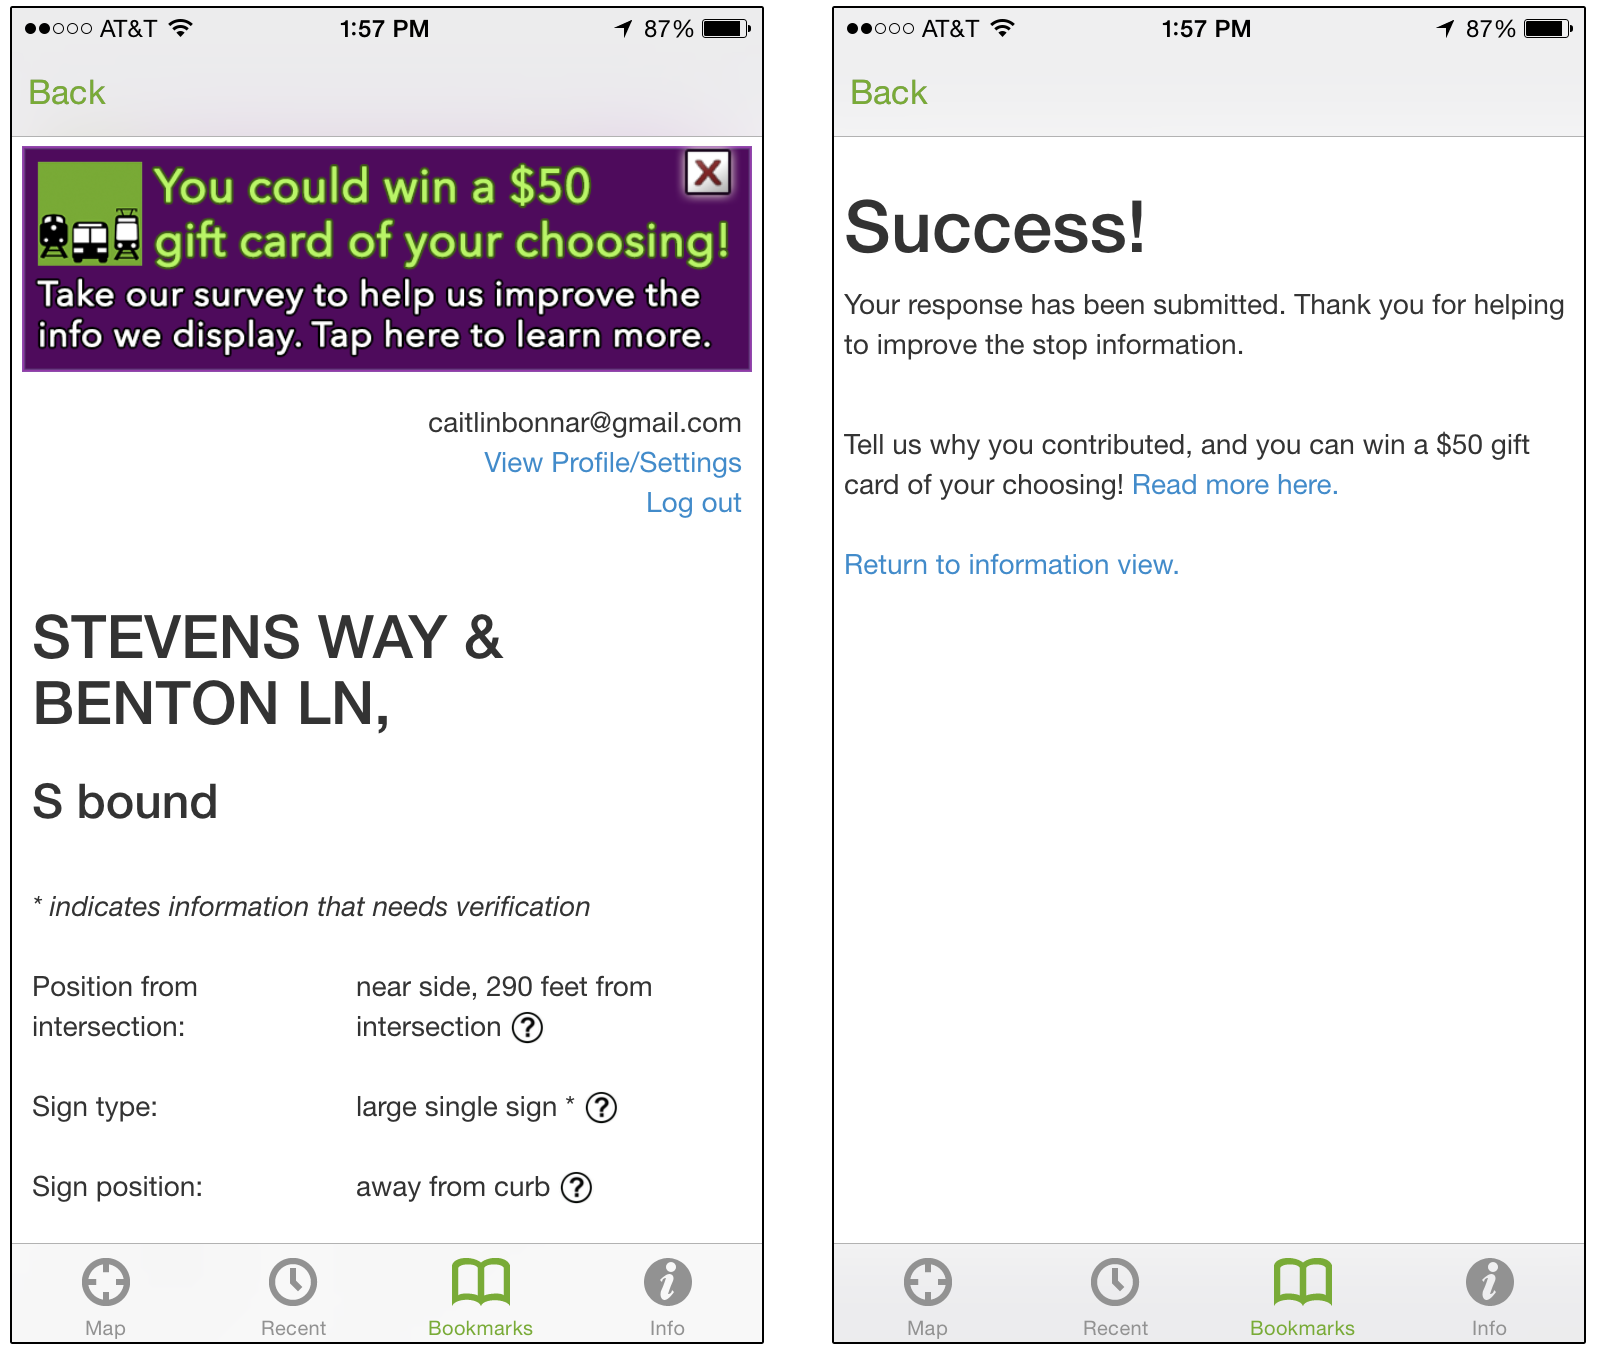
\includegraphics[width=.5\textwidth]{SurveyAlerts.png}
\caption{Screenshots of the survey recruiting methods we placed within the StopInfo application itself. The left screenshot includes a banner at the top of a stop's information page that the user can tap on to view the survey URL. The right screenshot includes the message that appears when a user submits information about a stop that also takes them to the survey URL.}
\label{fig:alerts}
\end{figure} 

\subsubsection{On-line Survey}
To begin the empirical investigation we created an on-line survey for both StopInfo contributors and non-contributors (primarily those who are frequent public transit riders and OneBusAway users). The survey includes structured questions based on some of the values identified in the harms and benefits analysis, as well as open-ended questions that allow for unstructured feedback. The survey was laid out as follows (each item corresponds to a different page of the survey):

\begin{enumerate}[leftmargin=8mm]
\item A consent page that informed them of the purpose of our study
\item Questions about public transit and OneBusAway usage
\item An overview of the StopInfo system including screenshots and a link to the live user interface, what information we collect from contributors, and the goal of the project
\item A question asking whether they have previously contributed to StopInfo
\item A list of open-ended questions about their motivations for contributing and concerns with the current system
\item Structured questions (answered on a 5-point Likert scale) about why they might or might NOT contribute 
\item Both structured and unstructured questions about potential new features and designs of the StopInfo system (including what information they would feel comfortable or uncomfortable with being collected or displayed as part of contributing)
\end{enumerate}

\begin{figure*}[t]
\centering
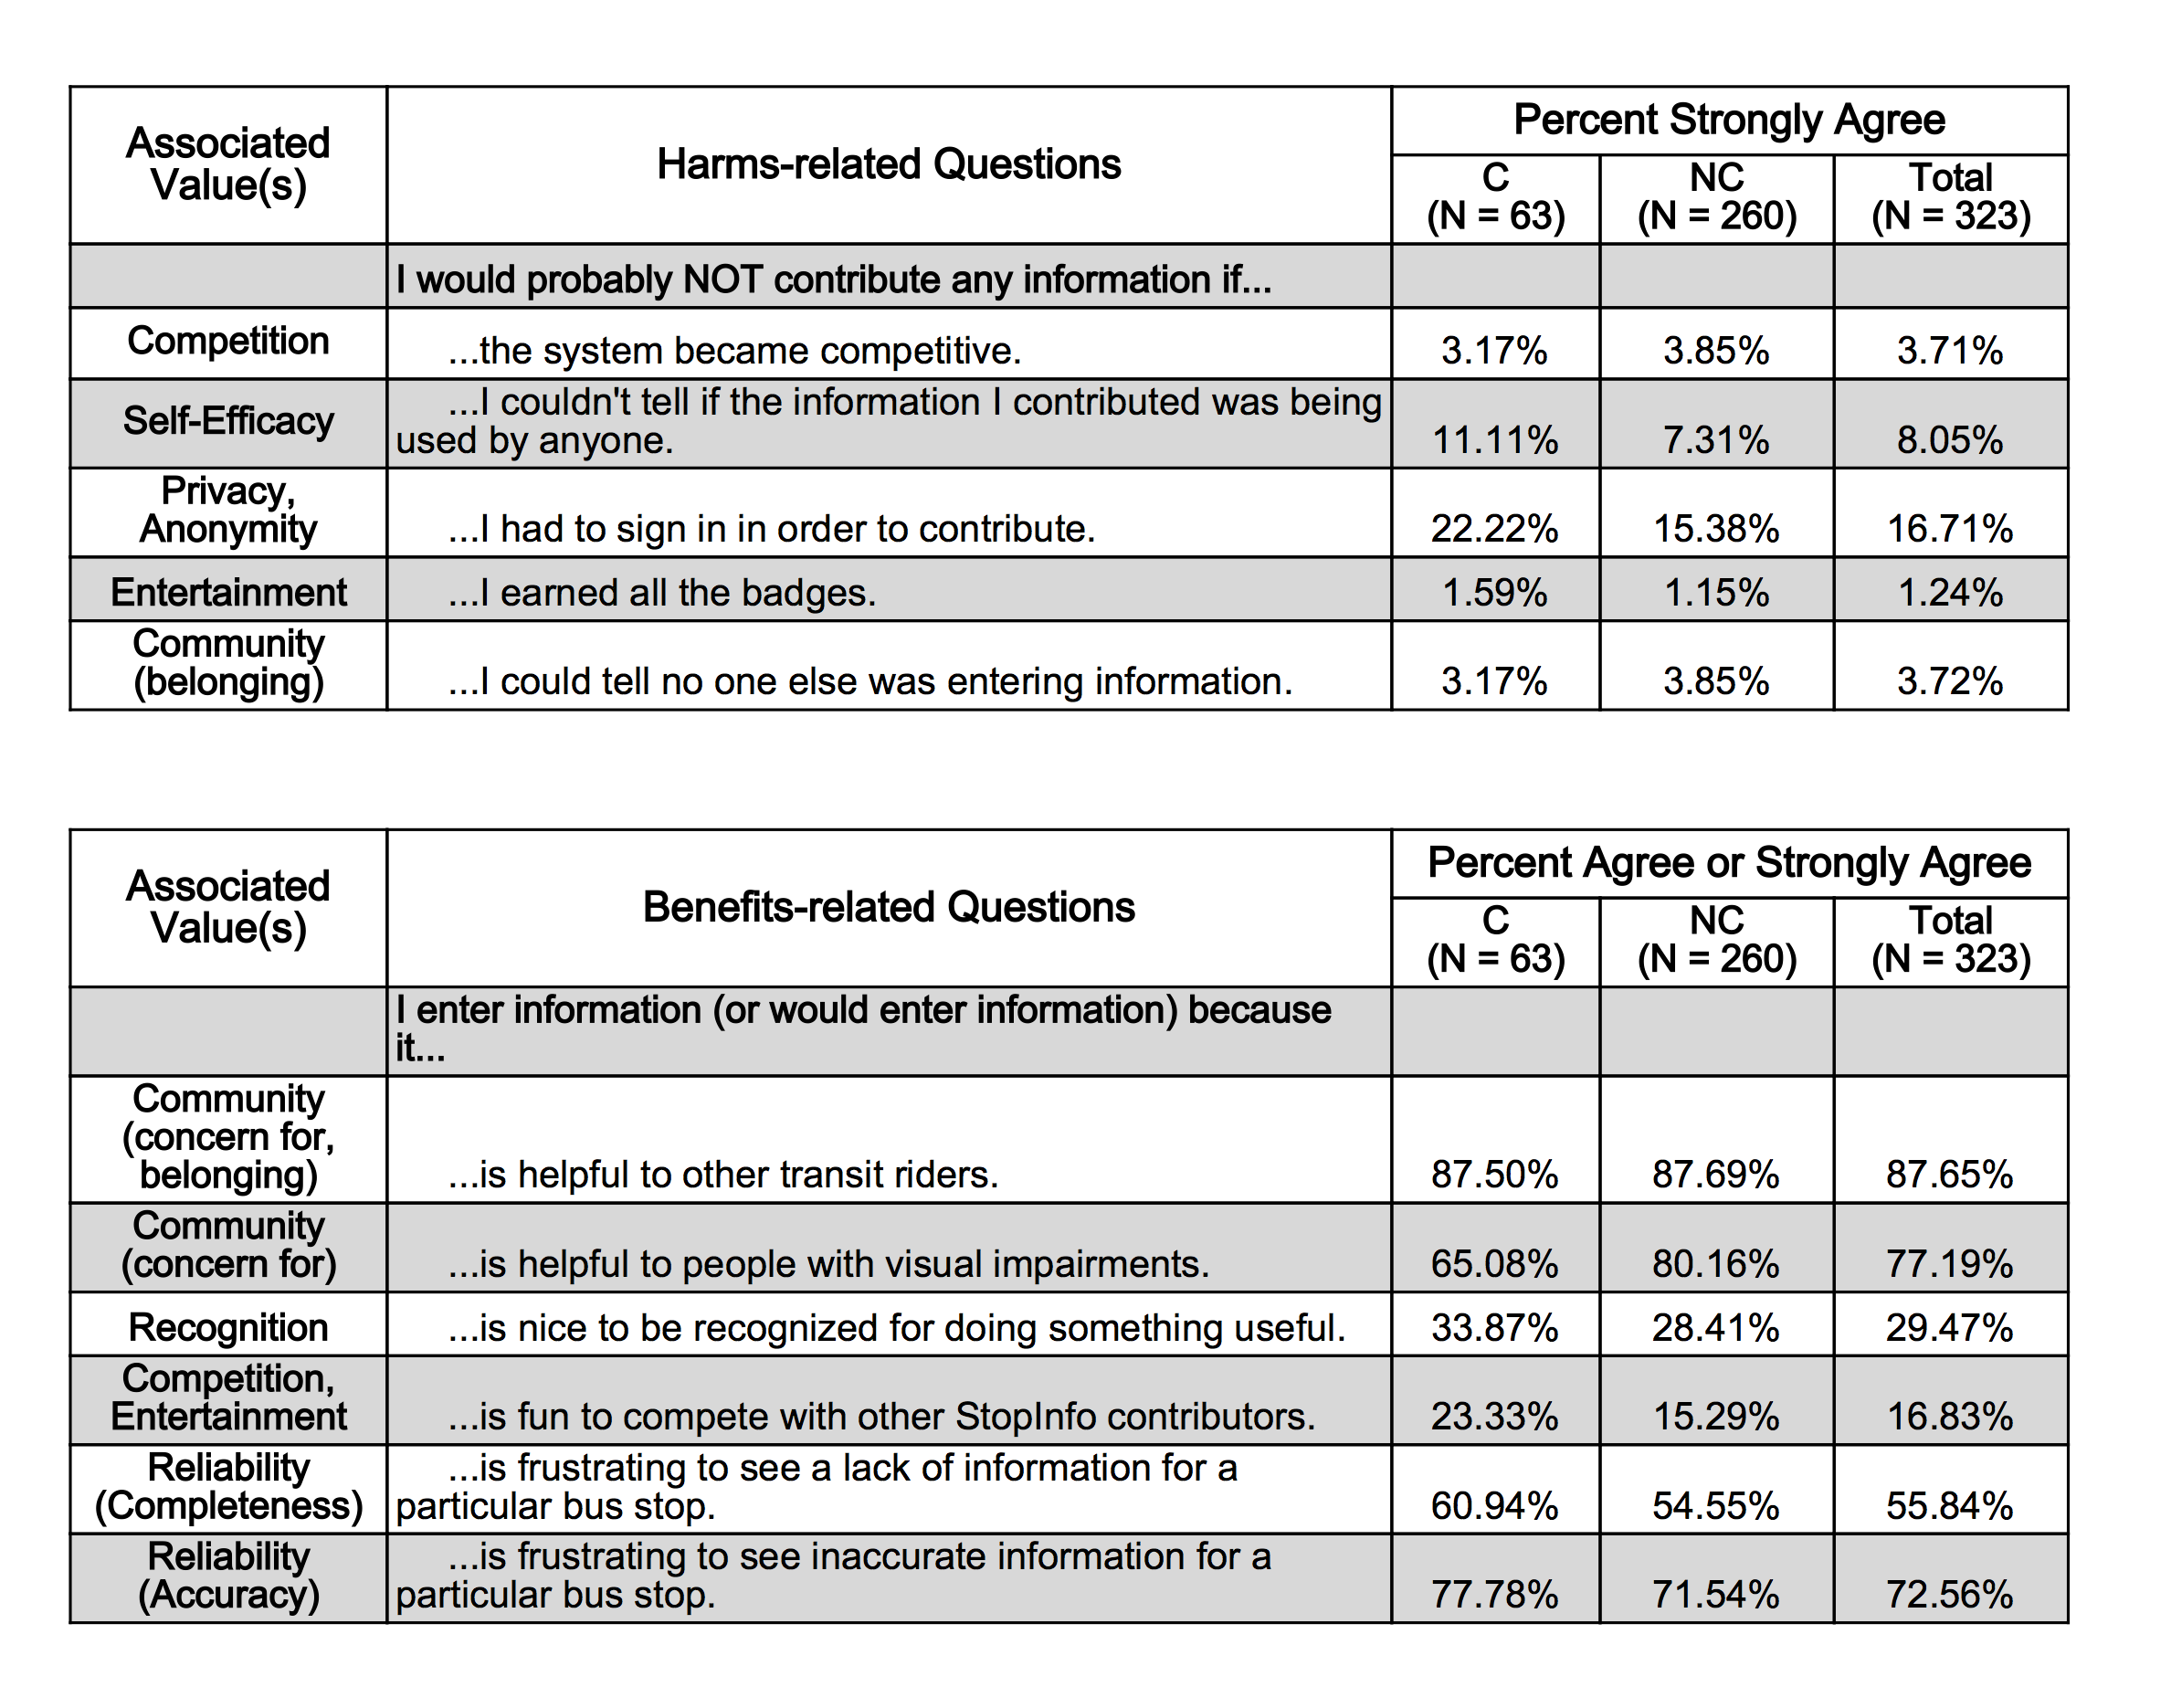
\includegraphics[width=\textwidth]{Results.png}
\caption{Selected preliminary survey results. Here we are considering both previous contributors to the StopInfo system (C, \emph{N} = 63) as well as non-contributors who indicated they would possibly be willing to contribute (NC, \emph{N} = 260). We exclude respondents who said they would likely never contribute (\emph{N} = 79) and those who did not disclose (\emph{N} = 8).}
\label{fig:results}
\end{figure*} 

As part of our structured questions on page six, we sought to distinguish who was meant by `community' by distinguishing between three different groups: other transit riders in the Seattle area, the transit agencies in the Seattle area that maintain the stops, or the community of blind and low vision people. We also sought to distinguish the differences between people's comfort with providing certain types of information (such as their name, e-mail address, GPS location, and the stops they've contributed to) by having them consider two types of systems: an \emph{opt-out} system, where this information is automatically collected unless they explicitly change a setting to stop us from collecting it, and an \emph{opt-in} system, where this information is NOT collected unless they explicitly change a setting that would allow us to collect it.

We deployed the survey by sending it out over a few local e-mail lists, posting it on a popular transit-oriented blog in Seattle, and creating an alert with a link to the survey within the OneBusAway iOS application, which is used by roughly 100,000 users in Puget Sound per week. We also placed an accessible banner that linked to the survey as well and posted a message asking contributors to take the survey after they submitted information for a stop within StopInfo itself (Figure \ref{fig:alerts}). To help incentivize participation, we offered the chance to win a \$50 gift card by allowing participants to enter their e-mail address at the end of the survey. 

We are still in the process of running the survey, but have so far gathered over 410 responses (54\% male, 42\% female) from both contributors and non-contributors to StopInfo. Table \ref{fig:results} shows some of the harms- and benefits-related questions on the survey along with a few preliminary results. These are some of the structured question on page six that ask to rate their agreement with certain statements according to a five-point Likert scale (ranging from ``Strongly Disagree'' to ``Strongly Agree). We present the results for both people who have previously contributed to StopInfo (the column labeled ``C'') as well as those who have not contributed to StopInfo before but had indicated that they would possibly contribute someday (the column labeled ``NC''). We also collected results for people who indicated that they had not contributed to StopInfo and likely never would, but we do not report them here as we are mostly interested in supporting the motives of those who are willing to contribute.

Following the Value Sensitive Design work of the CodeCOOP system by Miller et al. \cite{miller-2007}, we could also employ the Value Dam and Flow methodology in order to support the values of current contributors with features associated with value flows as well as help mitigate some of the concerns expressed by non-contributors (value dams). However, as we have not yet fully collected all of our responses, we have not yet determined threshold values to use for determining value dams and flows. Miller et al. use $\geq 50\%$ of agreement with benefits-related questions to be considered a value flow and  $\leq10\%$ strong agreement with harms-related questions to be considered a value dam. These values may also hold for our work, but further analysis is yet needed.

\pagebreak

\subsubsection{Semi-structured interviews}
At the end of the on-line survey, we asked participants if they would also be willing to participate in a follow-up phone interview with a member of our research team. The interviews were semi-structured and designed to last approximately 20 minutes. Interview questions address the main reason or reasons the participant has for contributing (or potentially contributing), any concerns they might have about the current system, who they wish to help impact with their submissions, potential designs of the request system, and their feelings on gamification of the system (i.e., the reputation system, badge system, and inclusion of an optional game). 

So far six interviews have been conducted (one female) with four contributors and two non-contributors. Results from these interviews are also forthcoming, however, one fact that stood out from many of these initial interviews is that knowing that the submitted information is directly useful to someone (especially if they are blind or low vision, as the interviewees perceived their value of the information to be greater than a sighted transit rider) would make them much more likely to submit information and/or sustain their contributions. For example, one contributor said that he did not previously know the goal of the system was to help blind and low vision transit riders locate stops, but \textit{``knowing that now, it definitely feels like adding the comments and being diligent about it, it makes me want to do it more, especially because it is going to benefit them directly.''}




